%Gran parte de esto lo generó el LyX
\documentclass[12pt,spanish]{article}
\usepackage{lmodern}
\usepackage[T1]{fontenc}
\usepackage[utf8]{inputenc}
\usepackage[a4paper]{geometry}
\geometry{verbose,tmargin=2cm,bmargin=2cm,lmargin=70pt,rmargin=70pt,headheight=35pt}
\usepackage{fancyhdr}
\pagestyle{fancy}
\usepackage{float}
\usepackage{textcomp}
\usepackage{graphicx}
\usepackage[spanish]{babel}
\usepackage{amsmath}

%Manejo de notas al pie; Captions en negrita en Figuras y Tablas
\usepackage[bottom]{footmisc}
\usepackage[hang,bf]{caption}
\usepackage{babel}
\addto\shorthandsspanish{\spanishdeactivate{~<>}}

%Incluir librería para listado código
\usepackage{xcolor,listings}

\lstset{
  literate={á}{{a}}1
           {é}{{e}}1
           {í}{{i}}1
           {ó}{{i}}1
           {ú}{{i}}1
}

%fuentes y colores
\lstset{
 belowcaptionskip=1\baselineskip,
  breaklines=true,
  frame=L,
  language=C,
  showstringspaces=false,
  basicstyle=\ttfamily\footnotesize,
  keywordstyle=\bfseries\color{green!30!black},
  commentstyle=\itshape\color{purple!30!black},
  identifierstyle=\color{blue},
  stringstyle=\color{orange},
  flexiblecolumns=true,
  numbers=left,                    % where to put the line-numbers; possible values are (none, left, right)
  numbersep=10pt,                   % how far the line-numbers are from the code
  numberstyle=\footnotesize, % the style that is used for the line-numbers
  tabsize=4,
}

\begin{document}

%Encabezado
\lhead{
\includegraphics[width=3cm]{logo-facu.jpg}}
\chead{}
\rhead{\textsc{Análisis numérico I} - 2do cuatrimestre de 2013\\
TP Nº1 - Ávila Alterach (94950), Fernandez Lema (93410)}

%Carátula
\begin{titlepage}
\thispagestyle{empty} %No poner número de página en título

\begin{center}
	
\includegraphics[width=10cm]{logo-facu-grande.jpg}
	\vfill
	
	\huge{75.12 - Análisis Numérico I} \\
	\LARGE{Trabajo Práctico Nº1 \\ Resolución de Sistemas de Ecuaciones Lineales}
	\vfill
	
	\normalsize{
	\begin{tabular}{lll}
		\textbf{Nombre} & \textbf{Correo electrónico} & \textbf{Padrón} \\ \hline 
		Gonzalo Ávila Alterach & gonzaloavilaalterach@gmail.com & 94950 \\
		Nicolás Mariano Fernandez Lema & nicolasfernandezlema@gmail.com & 93410 \\
	\end{tabular}
	}
	\vfill
		
	\large{Fecha de entrega: 16 de octubre \\ 2º cuatrimestre de 2013}
	\vfill
\end{center}
\end{titlepage}
\pagebreak

\section*{Resumen}
En este problema, el sistema a resolver se trata de $Ax=b$ , siendo A una matriz cuadrada tridiagonal, de dimensiones $(n-1)^2$.

El vector incógnita $x$ a averiguar está formado por los elementos $(c_1, c_2, ..., c_{n-1})$, ya que sabiendo su valor se pueden hallar el resto de los coeficientes de todos los polinomios.
Debido a las ecuación 4 y la 7, se puede apreciar que la matriz A es tridiagonal, y sus elementos son lo siguientes:

\[
A_n=
  \begin{pmatrix}
   2(h_0+h_1) & h_1 & 0 &  0 & \cdots & 0 & 0 &\\
   h_1 & 2(h_1+h_2) & h_2 & 0 &  \cdots & 0 & 0 &\\
   0 & h_2 & 2(h_2+h_3) & h_3  &  \cdots & 0 & 0 &\\
   \vdots  & \vdots & \vdots & \vdots & \ddots & \vdots & \vdots &\\
   0 & 0 & 0 & 0 & \cdots & h_{n-1} & 2(h_{n-1}+h_n)\\
  \end{pmatrix}
\]

Además, debido a que los datos de entrada utilizados la diferencia entre los $\theta _k$ consecutivos es constante, los $h_k$ también lo son, y por lo tanto la matriz queda simétrica.

Los programas se desarrollaron para resolver matrices genéricas, sin tener en cuenta que los sistemas del problema a resolver son tridiagonales, por lo que es una resolución muy ineficiente: se esta utilizando más memoria que la necesaria y también se están multiplicando muchas veces ceros por ceros.

\section*{Polinomios encontrados}
Las coeficientes $c_k$ encontrados, así como el resto de los coeficientes de los polinomios están en el apéndice A.
\section*{Radios espectrales}
Utilizando la estimación dada, dividir el error relativo de una iteración respecto de la anterior, los radios espectrales son los siguientes:

\subsection*{Día 1}
    \begin{tabular}{| l | l | l | l |}
    \hline
    Iteración & $\rho_J$ & $\rho_{GS}$ \\ \hline
1 & 0.365217 & 0.262669 \\
2 & 0.363875 & 0.280345 \\
3 & 0.445632 & 0.291762 \\
4 & 0.385874 & 0.288134 \\
5 & 0.49069 & 0.263809 \\
6 & 0.411277 & 0.317298 \\
7 & 0.480461 &  \\
8 & 0.431252 & \\ 
    \hline
    \end{tabular}

\subsection*{Día 2}
    \begin{tabular}{| l | l | l | l |}
    \hline
    Iteración & $\rho_J$ & $\rho_{GS}$ \\ \hline
1 & 0.336795 & 0.294195 \\
2 & 0.31415 & 0.299836 \\
3 & 0.482199 & 0.296196 \\
4 & 0.397669 & 0.295461 \\
5 & 0.475701 & 0.295959 \\
6 & 0.442331 & 0.296806 \\
7 & 0.462645 &  \\
8 & 0.464795 & \\ 
    \hline
    \end{tabular}

\subsection*{Día 3}
    \begin{tabular}{| l | l | l | l |}
    \hline
    Iteración & $\rho_J$ & $\rho_{GS}$ \\ \hline
1 & 0.156788 & 0.250333 \\
2 & 0.309514 & 0.255578 \\
3 & 0.375905 & 0.247174 \\
4 & 0.472542 & 0.245682 \\
5 & 0.469129 & 0.302341 \\
6 & 0.464291 & 0.283305 \\
7 & 0.473524 &  \\
    \hline
    \end{tabular}

\subsection*{Día 4}
    \begin{tabular}{| l | l | l | l |}
    \hline
    Iteración & $\rho_J$ & $\rho_{GS}$ \\ \hline
1 & 0.237237 & 0.261134 \\
2 & 0.430469 & 0.282262 \\
3 & 0.387289 & 0.281608 \\
4 & 0.486819 & 0.276875 \\
5 & 0.432466 & 0.317498 \\
6 & 0.485886 & 0.306247 \\
7 & 0.461146 &  \\
8 & 0.476161 &  \\
    \hline
    \end{tabular}
\\
\\
Debido a que la matriz es tridiagonal, deberia cumplirse la propiedad  $\rho_J ^2 = \rho_{GS}$. Sin embargo, se observa que el $\rho_{GS}$ es aproximadamente un 30\% mayor que lo esperado. Suponemos que esto se debe a que la estimación del radio espectral solamente sirve para ciertas matrices y condiciones particulares, y que es más precisa para iteraciones i más grandes.

Se realizó un pequeño script en Octave (se incluye en el apéndice C) para calcular el radio espectral real de la matriz de la iteración de Jacobi y la de Gauss Seidel. Dichos radios hallados son aproximadamente 0,5 para la de Jacobi y 0,25 para la de Gauss Seidel. Observando los radios espectrales estimados, es posible ver que la estimación del $\rho_J$ es bastante bueno (en las últimas iteraciones hay una diferencia pequeña entre lo esperado y lo calculado), mientras que la estimación del $\rho_{GS}$ es muy distinta a la esperada. Esto explica por qué Gauss Seidel no esta convergiendo en la mitad de las iteraciones que Jacobi.

\section*{Sobre relajación sucesiva}
Debido a que la matriz del sistema es tridiagonal, hay una fórmula para calcular el omega óptimo: 
$\omega _{opt} = {2 \over {1+ \sqrt{1-\rho_{TGS}}}}$

Utilizando los valores obtenidos experimentalmente de la sección anterior ($\rho_{TGS} \approx 0,3$) se obtiene un omega óptimo de aproximadamente 1,089.

Para calcular el mejor valor de omega, se iteró para todo $\omega$ entre 0,1 y 1,9, guardando cuantas iteraciones hizo falta para llegar a la convergencia con RTOL < 0,001.
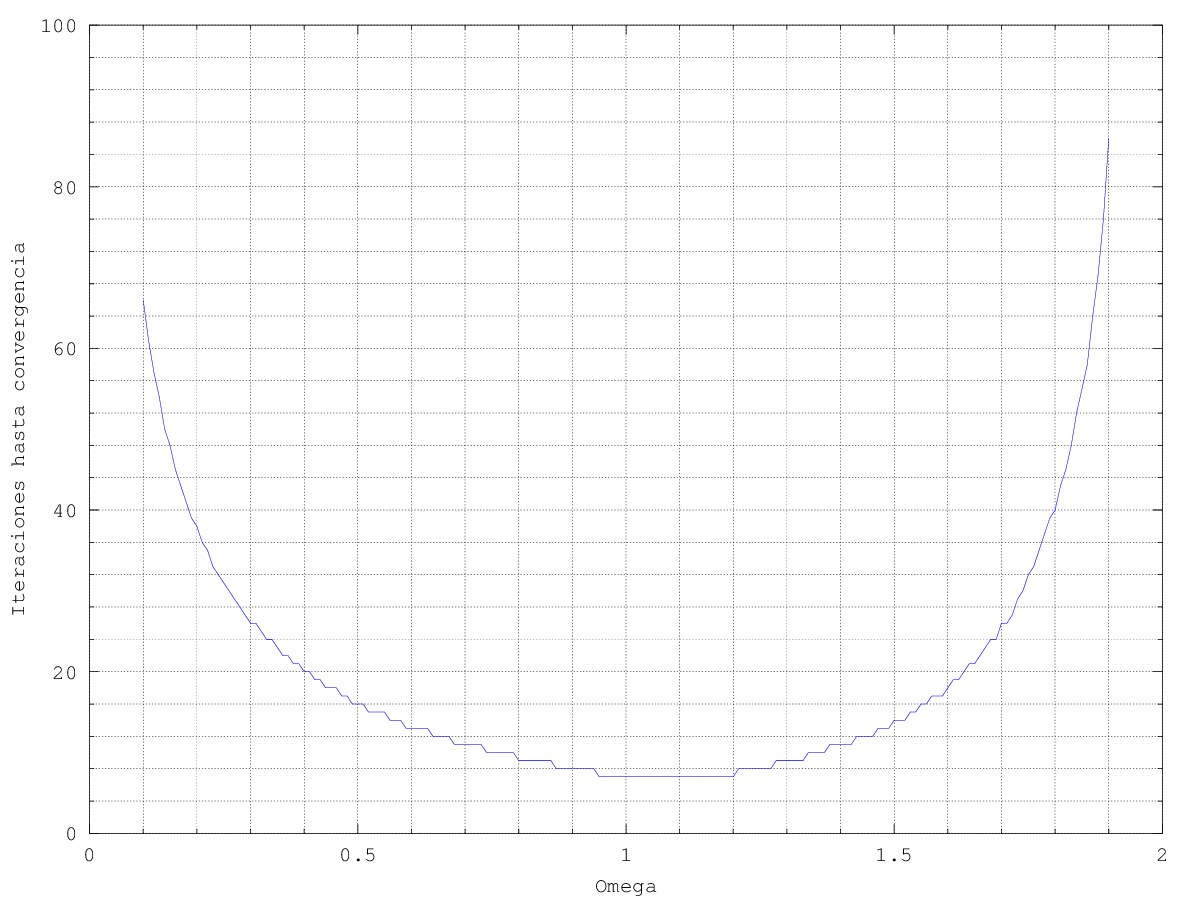
\includegraphics[scale=0.8]{../extras/omega.png}
Se puede observar que el gráfico corresponde con lo esperado, habiendo un mínimo absoluto para $\omega \approx 1.1$.

\section*{Gráfico de splines obtenidos}
Se utilizó como referencia de 0º el eje vertical, y ángulo aumentando en sentido horario.
Para evitar tener una curva abierta, se repitió el primer punto. Debido a la no inclusión de condiciones para mantener continuidad de la derivada entre el principio y el final, es posible ver que en $\rho$ = 0º la curva no es suave.
\subsection*{Día 1}
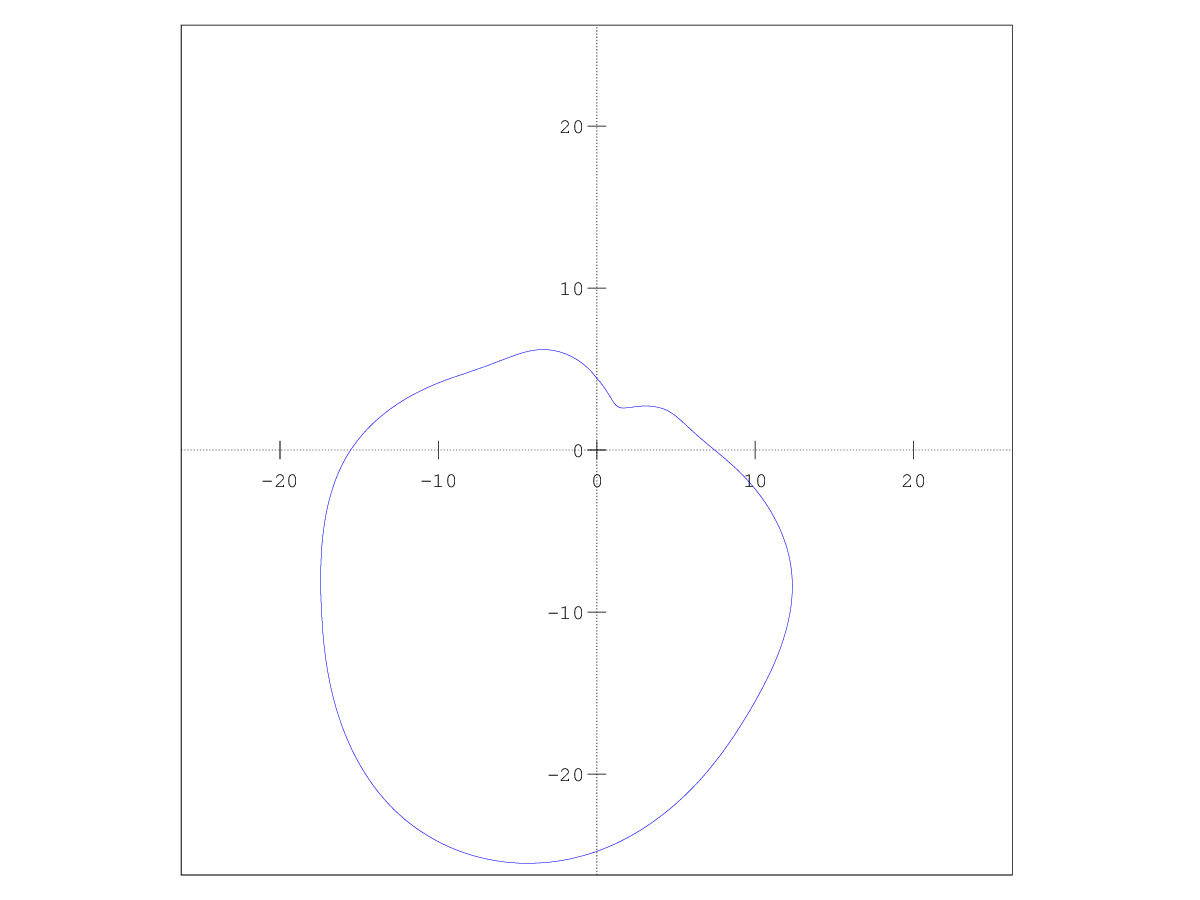
\includegraphics[scale=0.7]{../salida/dia1.png}
\subsection*{Día 2}
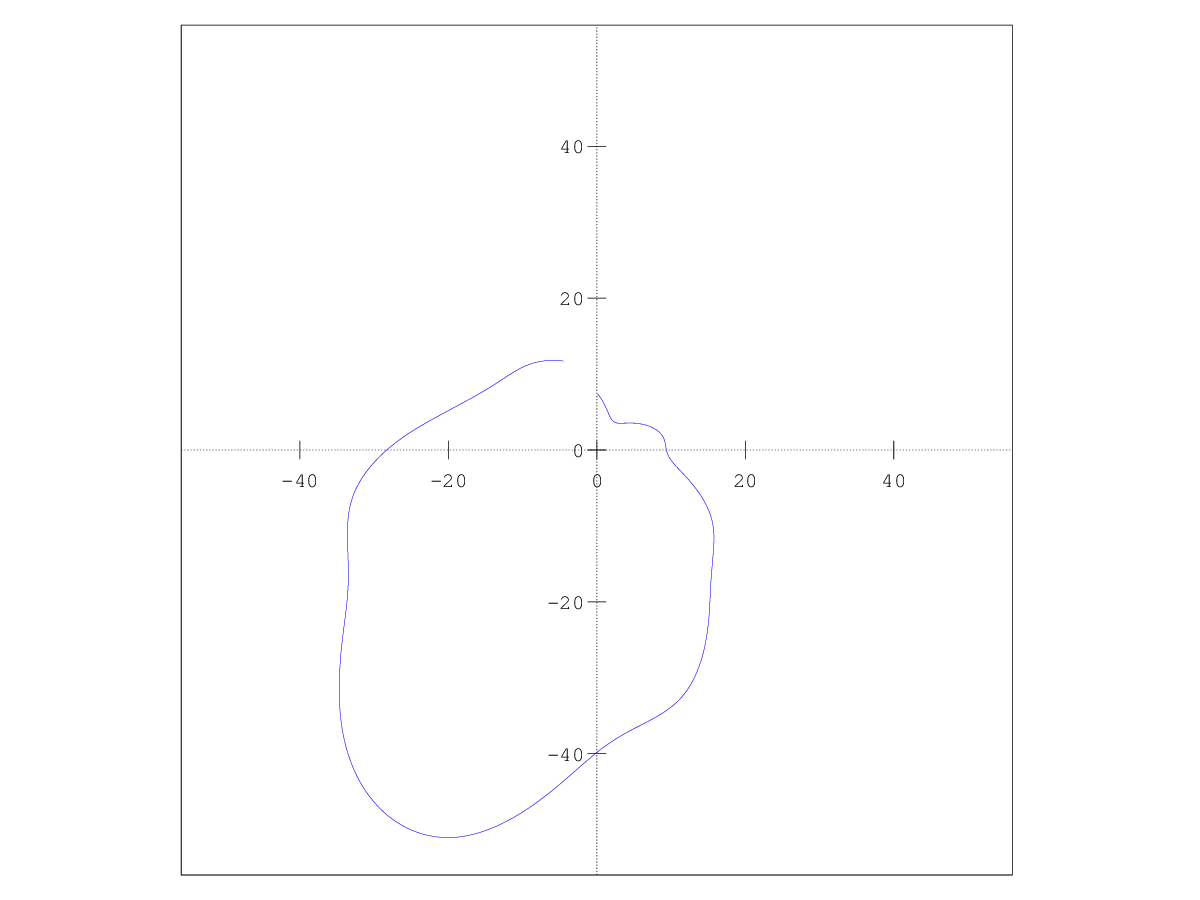
\includegraphics[scale=0.7]{../salida/dia2.png}
\subsection*{Día 3}
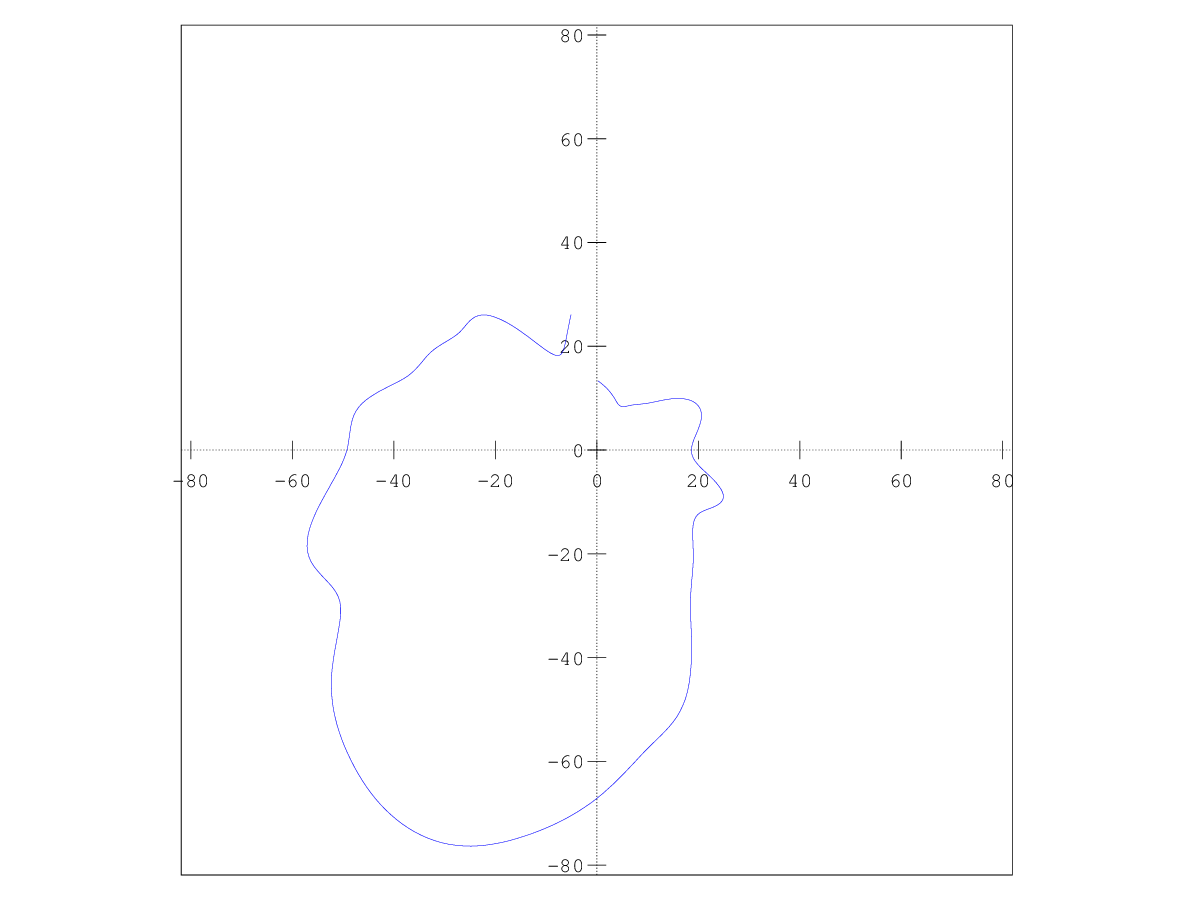
\includegraphics[scale=0.7]{../salida/dia3.png}
\subsection*{Día 4}
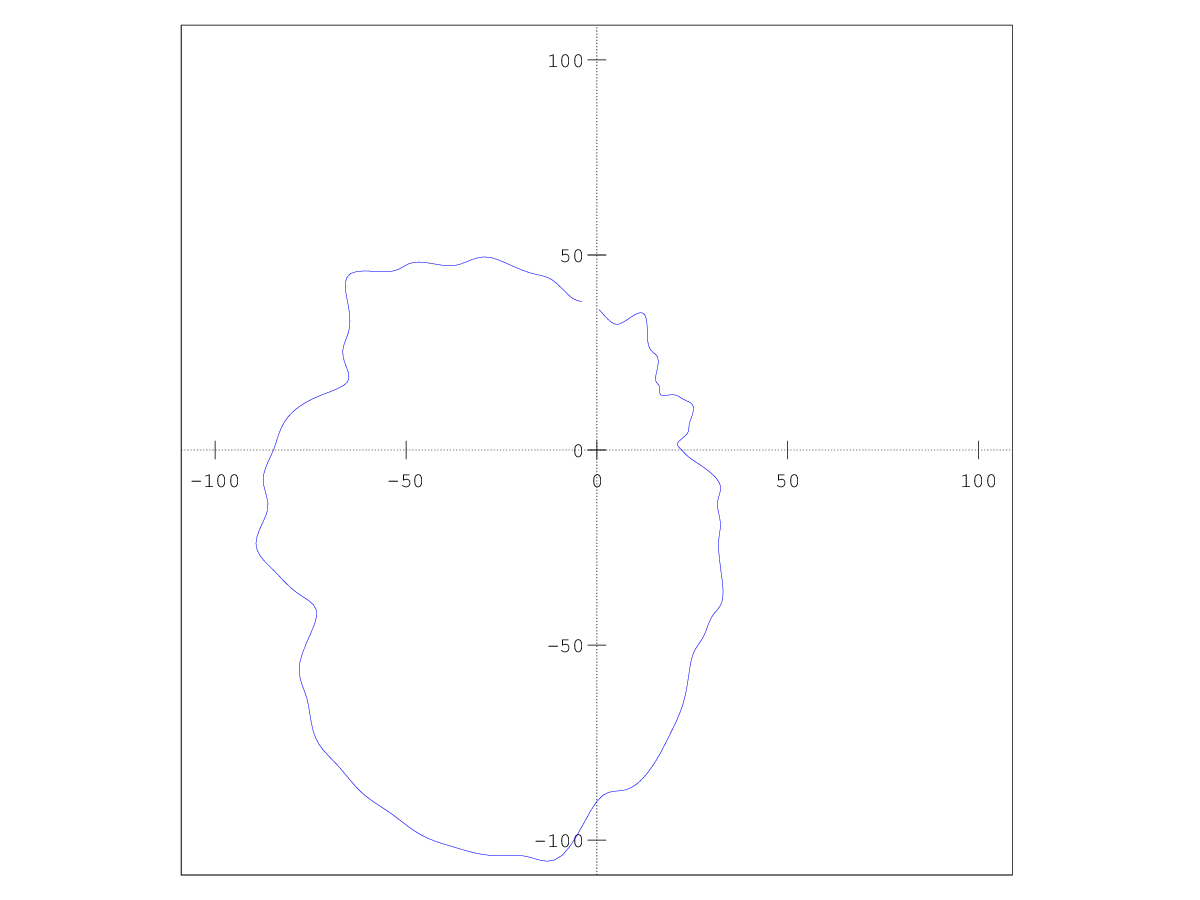
\includegraphics[scale=0.7]{../salida/dia4.png}

\section*{Máxima velocidad de avance}
La velocidad máxima de avance del fuego fue calculada observando la diferencia entre los radios de dos dias consecutivos, y encontrando el ángulo para el cual el radio varía la mayor cantidad entre el primer y el ultimo dia (en módulo).
Para esto se hizo un excel con los valores de dichos dias, se calculo la diferencia y se encontro el mayor.
Esto es a los 205º tubo una diferencia en su radio de aproximadamente 83, con esto podemos decir que la maxima velocidad del incendio es de 21 por dia.
Su direccion es en el angulo indicado, en nuestro grafico seria al sudoeste, y hacia afuera. 

\section*{Vivienda alcanzada por el fuego}
Se busca saber si una vivienda en una posicion dada es alcanzada por el fuego.
Para averiguar esto primero hay que ver en los cuatro días cuales fueron los radios del fuego en el ángulo de la casa: si siempre fueron menores entonces la casa no fue alcanzada por el fuego.

Si en algún día el radio del fuego es mayor al de la casa entonces la misma fue alcanzada por el fuego. Para saber en que tiempo fue alcanzada utilizamos una interpolacion lineal con los radios del fuego entre el dia que no fue alcanzada y el dia que fue alcanzada. Es decir, se asume que la velocidad del fuego es constante para un ángulo dado.

En nuestro caso la casa estaba hubicada en las coordenadas (188,36º; 94,18). La misma fue alcanzada por el fuego entre los días 3 y 4, con radio de 73,942 y 106,11 respectivamente.
Entonces el momento en que fue alcanzado por el fuego es: $t \approx (94,18 - 73,942)/(106.11 - 73.942) = 0.62903$.
Expresado en días y horas, la casa fue alcanzada aproximadamente el día 3 a las 15 hs.

\section*{Conclusiones}
El problema físico era analizar el frente de llama de un incendio, utilizando como datos mediciones discretas separadas un cierto ángulo entre si. El problema numérico era interpolar los datos para poder analizar la posición de las llamas entre dos mediciones. El método utilizado, los splines, en este caso la interpolación segmentaria cúbica plantea un sistema lineal para hallar los coeficientes de los polinomios. 

En este caso, dicho sistema lineal se resolvió mediante métodos iterativos: Jacobi, Gauss Seidel y SOR. Como la matriz del sistema es simétrica, tridiagonal, diagonal dominante, la convergencia de dichos métodos esta garantizada.

Como se esperaba por ser tridiagonal, el método de Jacobi converge en más iteraciones que Gauss Seidel. Además, SOR permite mejorar la convergencia, forzando los valores. En este caso, debido a que el omega óptimo no está tan alejado del 1, no hay tanta diferencia en cuanto a iteraciones hasta la convergencia entre Gauss Seidel y SOR. 

Los tipos de errores involucrados son los siguientes:
\begin{itemize}
    \item Errores de entrada: son los que provienen de las incertezas en las mediciones de los radios del fuego.
    \item Errores de truncamiento: debido a que no se pueden hacer infinitas iteraciones de los métodos, las soluciones obtenidas no son las soluciones exactas.
    \item Errores de redondeo: es el error por trabajar en un una computadora, utilizando tipos de datos con precisión finita. Se manifiesta en cada operación pero en este problema es muchos órdenes de magnitud menor al error de truncamiento.
    \item Errores del modelo matemático: es el error causado por el modelo en sí, en este caso sería que la interpolación spline no aproxime correctamente al frente de llama entre dos mediciones.
\end{itemize}

\newpage
\appendix
\section{Código (C++)}
\lstinputlisting[language=C++,texcl=true]{../tp1.cpp}
\section{Código para el calculo de W optimo (Octave/MATLAB)}
\lstinputlisting[language=MATLAB,texcl=true]{../extras/calculoOmegaOptimo.m}

\end{document}
